\documentclass[11pt]{article}
\usepackage{geometry}                % See geometry.pdf to learn the layout options. There are lots.
\geometry{letterpaper}                   % ... or a4paper or a5paper or ... 
%\geometry{landscape}                % Activate for for rotated page geometry
%\usepackage[parfill]{parskip}    % Activate to begin paragraphs with an empty line rather than an indent
\usepackage{graphicx}
\usepackage{amssymb}
\usepackage{commath}
\usepackage{amsmath}
\usepackage{epstopdf}
\usepackage{subfigure}
\usepackage[colorlinks=true, pdfstartview=FitV, linkcolor=black, citecolor=black, urlcolor=blue]{hyperref} % to be able to hyperlink to figures, etc, in text
\usepackage{natbib} % for better bibliography referencing. \citet without parentheses and \citep with them%
%\usepackage{fancyvrb} % This is to be able to make boxes around verbatim code in figures
% The following are to be able to go to smaller heading than subsubsection. Use "paragraph" and then "subparagraph"
\setcounter{secnumdepth}{5} % to be able to use more section headings
% here are the section headings in order to use in the text:
%\section{} % level 1
%\subsection{} % level 2
%\subsubsection{} % level 3
%\paragraph{} % level 4 - equivalent to subsubsubsection
%\subparagraph{} % level 5
%%%
\setcounter{tocdepth}{5} % To include all of the section headings in the table of contents
\DeclareGraphicsRule{.tif}{png}{.png}{`convert #1 `dirname #1`/`basename #1 .tif`.png}

\title{Oil Tracking on the TX-LA Shelf}
\author{Kristen M. Thyng}
%%\date{January 27, 2011}                                           % Activate to display a given date or no date

% 
% a few handy macros

\newcommand\matlab{{\sc matlab}}
\newcommand{\goto}{\rightarrow}
\newcommand{\bigo}{{\mathcal O}}
\newcommand{\half}{\frac{1}{2}}
%\newcommand\implies{\quad\Longrightarrow\quad}
\newcommand\reals{{{\rm l} \kern -.15em {\rm R} }}
\newcommand\complex{{\raisebox{.043ex}{\rule{0.07em}{1.56ex}} \hskip -.35em {\rm C}}}


% macros for matrices/vectors:

% matrix environment for vectors or matrices where elements are centered
\newenvironment{mat}{\left[\begin{array}{ccccccccccccccc}}{\end{array}\right]}
\newcommand\bcm{\begin{mat}}
\newcommand\ecm{\end{mat}}

% matrix environment for vectors or matrices where elements are right justifvied
\newenvironment{rmat}{\left[\begin{array}{rrrrrrrrrrrrr}}{\end{array}\right]}
\newcommand\brm{\begin{rmat}}
\newcommand\erm{\end{rmat}}

% for left brace and a set of choices
\newenvironment{choices}{\left\{ \begin{array}{ll}}{\end{array}\right.}
\newcommand\when{&\text{if~}}
\newcommand\otherwise{&\text{otherwise}}
% sample usage:
%  \delta_{ij} = \begin{choices} 1 \when i=j, \\ 0 \otherwise \end{choices}


% for labeling and referencing equations:
\newcommand{\eql}{\begin{equation}\label}
\newcommand{\eqn}[1]{(\ref{#1})}
% can then do
%  \eql{eqnlabel}
%  ...
%  \end{equation}
% and refer to it as equation \eqn{eqnlabel}.  


% some useful macros for finite difference methods:
\newcommand\unp{U^{n+1}}
\newcommand\unm{U^{n-1}}

% for chemical reactions:
\newcommand{\react}[1]{\stackrel{K_{#1}}{\rightarrow}}
\newcommand{\reactb}[2]{\stackrel{K_{#1}}{~\stackrel{\rightleftharpoons}
   {\scriptstyle K_{#2}}}~}

% Headers for exercises:

\newcommand{\exercise}[1]{\vskip 15pt  \noindent {\large \bf Exercise #1}%
     \nopagebreak\vskip 5pt \nopagebreak}

\newcommand{\chapexercises}[1]{%
     \cleardoublepage
     \centerline{\LARGE\bf Chapter #1 Exercises}
     \vskip .5cm
     \noindent
     From: {\it Finite Difference Methods for Ordinary and Partial 
     Differential Equations}\\  by R.~J.~LeVeque, SIAM, 2007.~~~
     {\tt http://www.amath.washington.edu/$\sim$rjl/fdmbook}
     \vskip .5cm
     }


%% Kristen's added
% Partial derivative d
\newcommand{\p}{\partial}
% integral dt
\newcommand{\dd}{\text{d}}
\newcommand{\ul}{\uvec{\ell}}
%\newcommand{\dx}{\text{dx}}
%\newcommand{\dy}{\text{dy}}
%\newcommand{\dr}{\text{dr}}
%\newcommand{\dl}{\text{d$\uvec{\ell}$}}
% Full partial derivative fraction, use like \pd[x]{t} for \frac{\partial x}{\partial t}
\newcommand{\pd[2]}{\frac{\partial #1}{\partial #2}}
% left and right big parentheses, \left{ and \right} as \lp and \rp
\newcommand{\lp}{\left(}
\newcommand{\rp}{\right)}
\newcommand{\uvec}{\underline} % for vectors
\newcommand{\uuvec[1]}{\underline{\underline #1 }} % for tensors
\newcommand{\ovec}{\overline} % for reynolds stresses

% Better tilde: http://tex.stackexchange.com/questions/9363/how-does-one-insert-a-backslash-or-a-tilde-into-latex
\newcommand{\ttilde}{{\raise.17ex\hbox{$\scriptstyle\sim$}}}

% \linenumbers % add line numbers

% \begin{frontmatter}

\begin{document}
\maketitle

\section{Introduction}

% Summarize literature on particle tracking, particularly applications of tracmass. Include potentially pitfalls and things to be aware of.
\subsection{Particle Tracking}


% How does the tracking code work in general?
\section{Tracking Algorithm Sensitivity and Details}

% Summarize tracmass and tracpy details
\subsection{Explain Algorithm}

\subsubsection{2D Boundaries}

Due to the basic algorithm of TRACMASS, at boundaries within the numerical domain, drifters will be stopped according to the bounding fluxes. For a given grid cell in the 2D case, there are four fluxes controlling a drifter's movement. Drifters have nonzero fluxes on active sides of the cell and zero fluxes along masked land. They can run along these walls but should not penetrate them. At open numerical boundaries, the drifters will be stopped according to a check built into tracmass itself, and will be left with their final position along the open boundary and a flag indicating that they have exited the domain so they will not be stepped forward.

The addition of subgrid turbulence parameterizations can affect this. One method is to add parameterized turbulent values to the fluxes used to calculate drifter movements. These do not affect the fact that fluxes will be zero at masked land because they are multiplied by the original ufluxes to get the fluctuation to add to the original flux values.

However, there are two methods of adding in a random walk to the particle positions directly, and these were affecting the boundary behavior of drifters near walls. The problem was that when a drifter was alongside a masked land cell, if the random new position of the drifter was just right to move the drifter from its current cell into the land cell, then an error check later in the code for the volume of the cell would catch the drifter (due to its cell having zero volume since it was on land) and the drifter would be stopped at its location near land. Since drifters in the advection-only and turbulent velocity methods do not hit land, the overall behavior was different along the coastline for the diffusion and anisodiffusion methods (in these methods, many more drifters were congregated alongshore). I changed this by adding a check in the diffusion subroutine in tracmass to not accept a new displacement location for a drifter if the layer thickness (dzt) of that new location is zero. Now, I think that all of the routines will have similar coastline behavior. If, on the other hand, it is desired that drifters should be able to hit the coastline and ``beach,'' then this behavior in the diffusion routines might be desired.

% Diffusion parameters and number of interpolation steps
\subsection{Examine Sensivity of Results to Input Parameters}

A series of numerical surface drifter experiments were run for 16 days forward in time from 11/20/2009 with several changing parameters to understand their importance to the results.

There is little overall difference for the number of time interpolation steps for these simulations (not shown).

The difference in the results from diffusion types is illustrated in Figure \ref{diffusiontype}. For numerical drifter experiments with drifters initially seeded 10 km apart and using the same horizontal diffusivity, the difference in tracks and final positions is not extreme, but is noticeable. The cases with no diffusion and parameterized turbulent velocities (Figures \ref{diffusiontype-none} and \ref{diffusiontype-turb}) are similar, though a larger value of $A_H$ would presumably change this more. The cases with a random walk-type diffusion added to the particle tracks themselves (Figures \ref{diffusiontype-aniso} and \ref{diffusiontype-diff}) show more diffused behavior and are fairly similar to each other.

\begin{figure}
    \centering
    \subfigure[No diffusion]{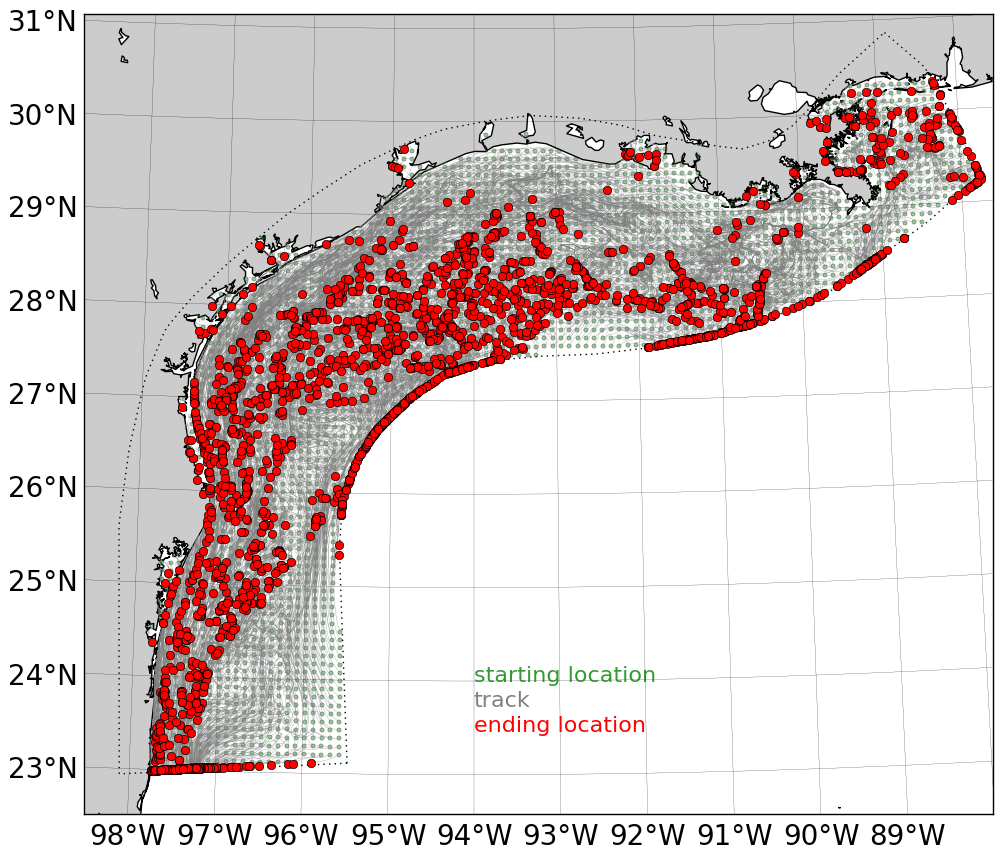
\includegraphics[width=.235\textwidth]{figures/sensitivity/10_5_None_Ftracks} \label{diffusiontype-none}}
    \subfigure[Turbulence]{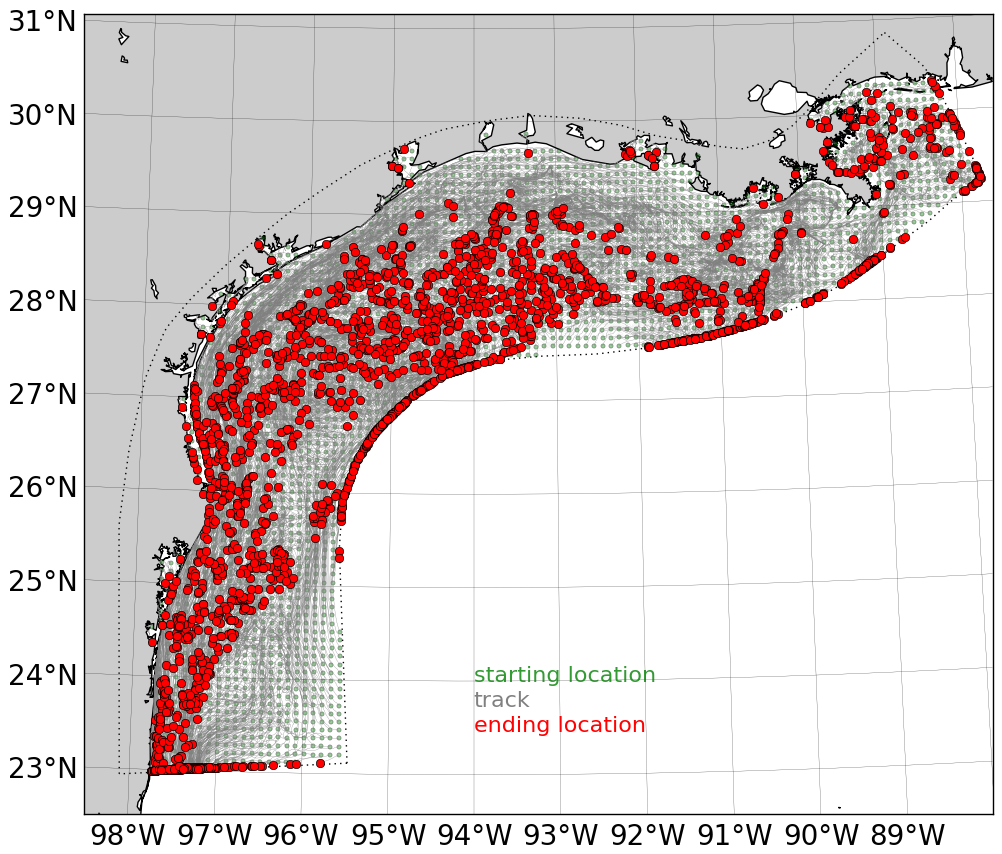
\includegraphics[width=.235\textwidth]{figures/sensitivity/10_5_Turb20_Ftracks} \label{diffusiontype-turb}}
    \subfigure[Elliptical]{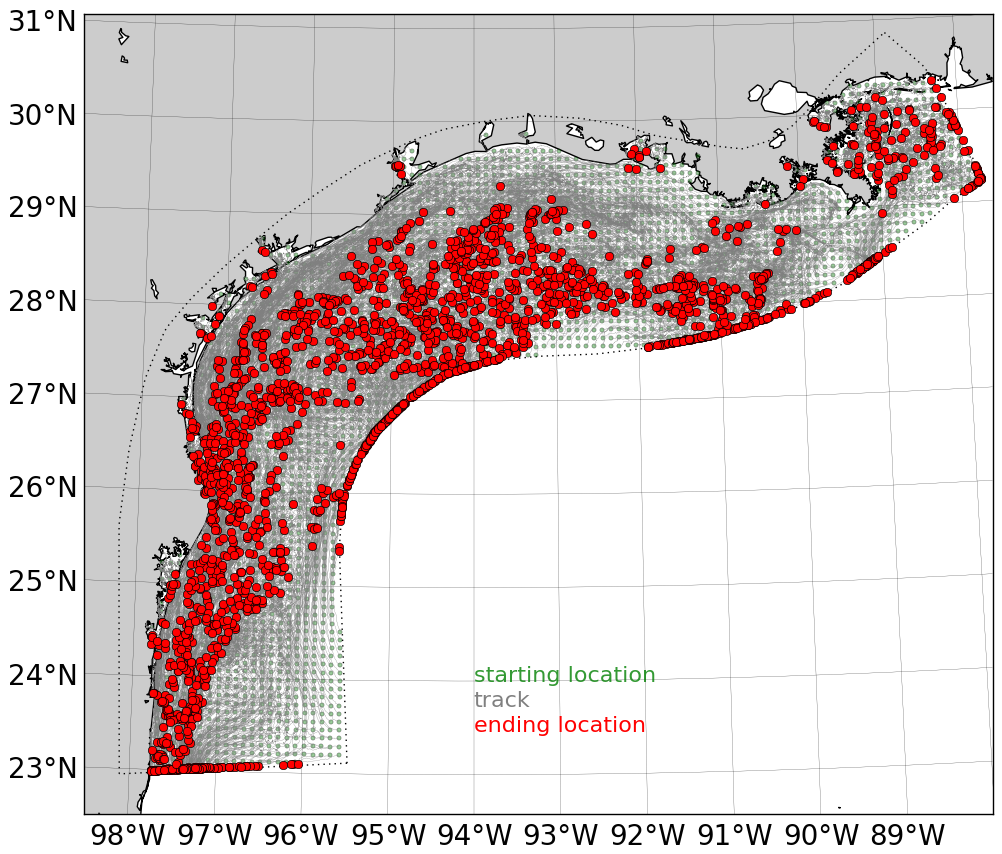
\includegraphics[width=.235\textwidth]{figures/sensitivity/10_5_A20_Ftracks} \label{diffusiontype-aniso}}
    \subfigure[Circular]{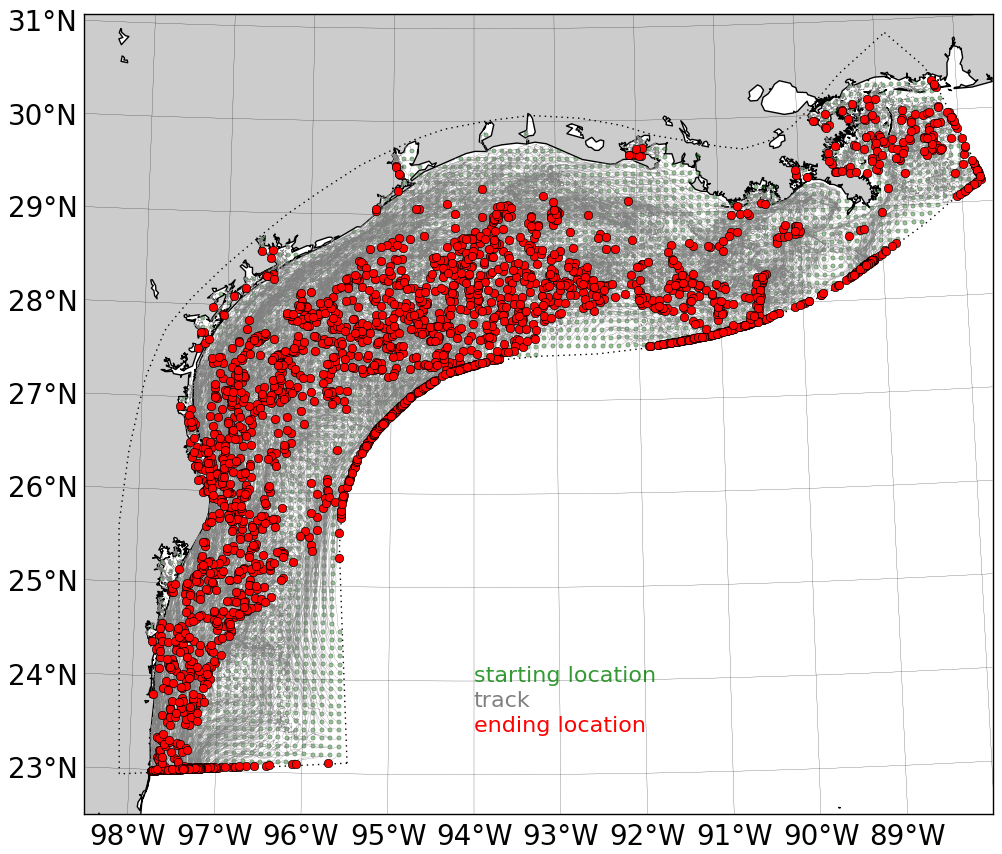
\includegraphics[width=.235\textwidth]{figures/sensitivity/10_5_D20_Ftracks} \label{diffusiontype-diff}}
    \caption{Comparison of types of diffusion for $A_H=20$ m$^2$/s, initial spacing of 10km}
    \label{diffusiontype}
\end{figure}

Drifter tracks and final locations are shown in Figure \ref{diffusionsize} for changing the size of the horizontal diffusivity, $A_H$. The overall behavior is the same in all of the plots, but the drifters are somewhat noticeably more spread out as the value of the horizontal diffusivity increases. This is shown for adding diffusion using a random walk on a circle to the drifter positions, but the same type of behavior is found in the results of all of the parameterization techniques (not shown).

\begin{figure}
    \centering
    \subfigure[No diffusion]{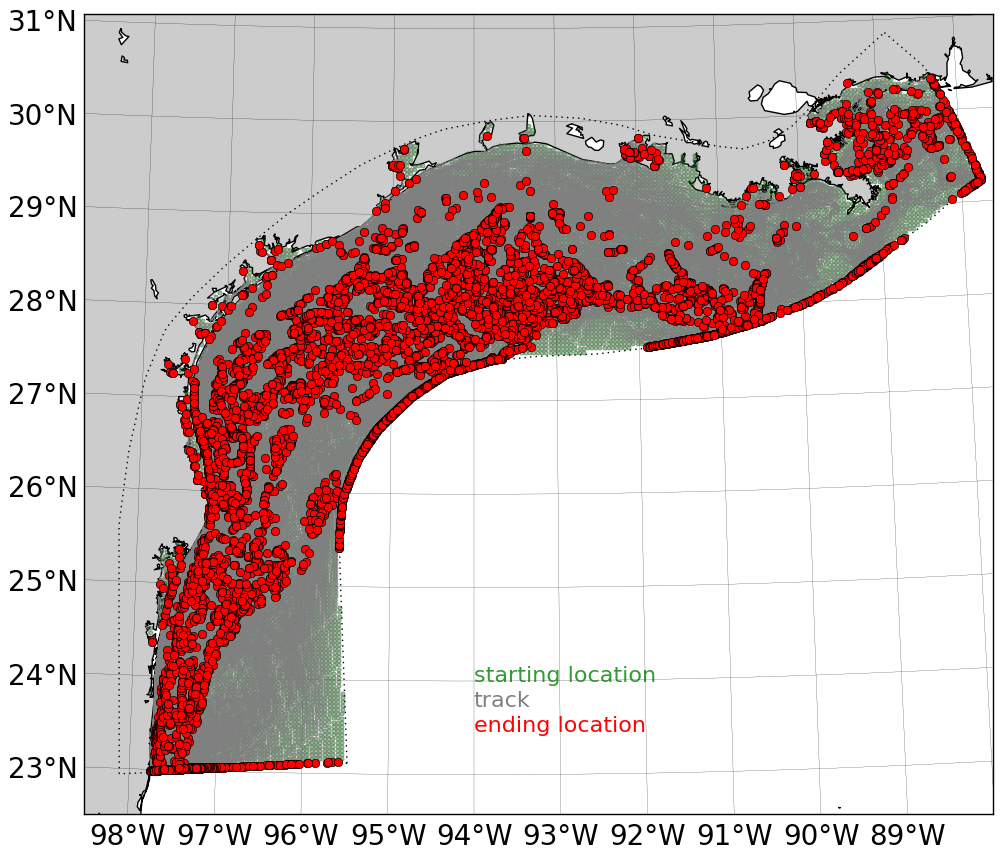
\includegraphics[width=.315\textwidth]{figures/sensitivity/5_5_None_Ftracks} \label{diffusionsize-none}}
    \subfigure[Circular diffusion, $A_H=5$]{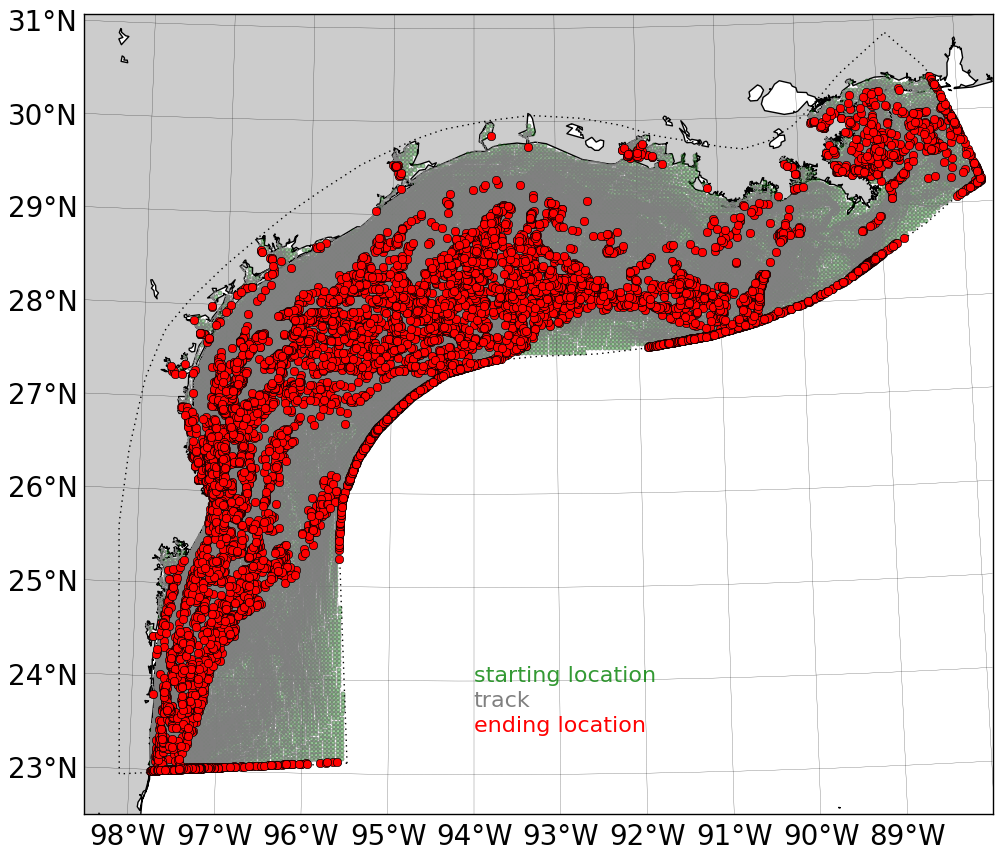
\includegraphics[width=.315\textwidth]{figures/sensitivity/5_5_D5_Ftracks} \label{diffusionsize-5}}
    \subfigure[Circular diffusion, $A_H=20$]{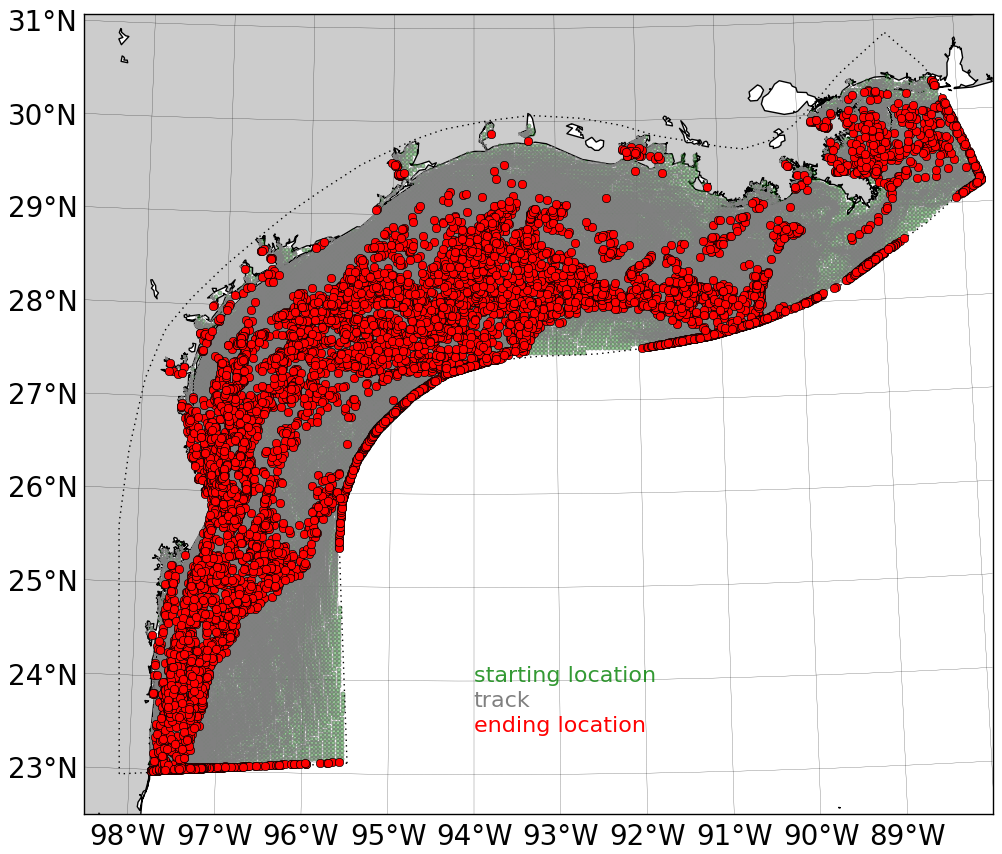
\includegraphics[width=.315\textwidth]{figures/sensitivity/5_5_D20_Ftracks} \label{diffusionsize-20}}
    \caption{Comparison of size of $A_H$ for initial spacing of 5km and circular trajectory diffusion}
    \label{diffusionsize}
\end{figure}



% \begin{figure}
%   \centering
%   \subfigure[Circular, 5 km spacing]{\includegraphics[width=.325\textwidth]{figures/5_5_D20_Fhistpcolor}}
%   \subfigure[Circular, 10 km spacing]{\includegraphics[width=.325\textwidth]{figures/10_5_D20_Fhistpcolor}}
%   \subfigure[Circular, 50 km spacing]{\includegraphics[width=.325\textwidth]{figures/50_5_D20_Fhistpcolor}}
%   \caption{Comparison of initial drifter spacing with diffusion ($A_H=20$ m$^2$/s.}
% \end{figure}


% Move drifters backward and forward from Galveston and compare
\subsection{Forward/Backward}


% How well does the particle tracking apply to the TXLA shelf?
\section{Performance of Model and Tracker}

% As in Blanke 1999, run drifters forward and backward and compare mass flux as validation
\subsection{Mass Flux Comparison}

% Gyre test: To evaluate tracker performance. Maybe also use older tracker as comparison.
\subsection{Gyre Test}

\subsection{Sensitivity to Waves, Tides, and Model Output Frequency}


\section{Drifter Transport} \label{sec:transport}

\subsection{Methodology}

The idea is to assign an initial volume transport property to the drifters based on their initial placement and velocity and, given a high enough density that the result does not change with more drifters, track the $x$ and $y$ transport as the drifters pass numerical grid cell walls. The initial volume transport is found by summing the overall flux into or out of the grid cells in which drifters are initially located and dividing by the number of initial drifters in the cells, or
\begin{align*}
    T_0 &= \frac{1}{N_0} \left(\left|u[i_0,j_0,k_0,t_0]\right| \Delta y_{i_0,j_0} \Delta z_{i_0,j_0,k_0,t_0} + \left|v[i_0,j_0,k_0,t_0]\right| \Delta x_{i_0,j_0} \Delta z_{i_0,j_0,k_0,t_0}\right),
\end{align*}
where $N_0$ is the number of drifters initialized in a grid cell or grid cells (in which case $N_0$ is a vector), $u[i_0,j_0,k_0,t_0]$ and $v[i_0,j_0,k_0,t_0]$ are the zonal and meridional velocities for the initial grid cell(s) at grid index locations $i_0,j_0,k_0$, the drifters are seeded at time $t_0$, and the grid cell spacing in the zonal and meridional directions is given by $\Delta x_{i_0,j_0}$ and $\Delta y_{i_0,j_0}$ (assuming they can change horizontally but not vertically or in time), and in the vertical direction is given by $\Delta z_{i_0,j_0,k_0,t_0}$ (which can change in all dimensions) \citep{Doos:1995tf}.

Assuming that all drifters that enter a grid cell will exit via another grid cell wall, the 3D transport field is non-divergent, that is,
\begin{align}
    \partial_i U + \partial_j V + \partial_k W &= 0, \label{transport}
\end{align}
for zonal, meridional, and vertical volume transports $U,V,W$ and directions $i,j,k$. Alternatively, this can be written in terms of the numerical discretization as:
\begin{align}
    U_{i,j,k,n} - U_{i-1,j,k,n} + V_{i,j,k,n} - V_{i,j-1,k,n} + W_{i,j,k,n} + W_{i,j,k-1,n} &= 0, \label{transport_discretized}
\end{align}
where $U_{i,j,k,n}, V_{i,j,k,n}, W_{i,j,k,n}$ are the $(x,y,z)$ volume transports registered for drifter instance $n$ for grid cell located at indices $(i,j,k)$. 

In this work, the vertical direction is assumed to be unimportant (these are surface-only drifters), so only the zonal and meridional directions are used. Everytime a drifter crosses a grid cell wall in the positive zonal or meridional direction, its initial volume transport (which is a property of the drifter) is registered at that cell wall by adding it to the running total. Drifters moving past a wall in a negative zonal or meridional direction are subtracted from the transport total at that wall. Thus, an array that is the size of the cell walls of the numerical grid for the $u$ direction and one for the $v$ direction is generated of the volume transport as represented by the drifters that pass the cell walls.  

\subsection{Results}

In this simulation, surface-restricted drifters were released at a location $(-88.5159,28.8881)$ near the Deepwater Horizonal Oil Spill $(-88.3659,28.7381)$ (the actual site is just outside the model domain). 100 drifters were seeded at the same location every four hours (due to the frequency of model output) from April 20, 2010 through July 15, 2010, to represent a fixed amount of material regularly moving away from the initial site, and followed forward in time for 90 days (with 5 interpolation steps between each model output). Subgrid scale effects were represented using an added random turbulence to the grid cell fluxes used to calculate the drifter paths, with a horizontal diffusion of $A_h=20$ m$^2$/s. Drifters were initialized with a volume transport, $T_0$, representing the initial flux out of the cells when they were released (divided by the number of drifters). This is used to track the transport of the drifters over all of the simulations together, to understand where the model predicts surface oil from the spill traveled. To present the information, the square root of the sum of the squares of the two components of volume flux on the grid is calculated. 

\begin{figure}
    \centering
    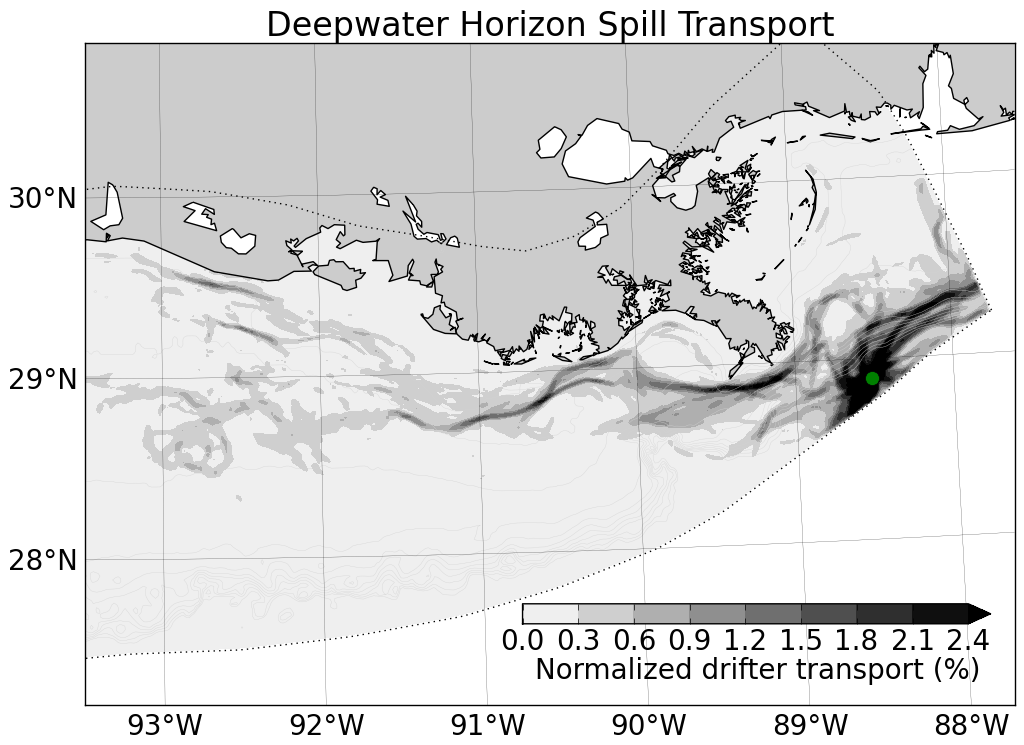
\includegraphics[width=\textwidth]{figures/dwh_stream_f/transport}
    \caption{Transport of surface material from a site representing the Deepwater Horizon oil spill (in green), as calculated from Lagrangian drifters. The transport values have been normalized by the volume transport represented by the drifters and multiplied by 100 to find percentage transport values. Note that the colorbar has been set to a lower value than the true maximum in order to demonstrate more transport paths than would otherwise by visible.}
    \label{fig:dwh_transport}
\end{figure}

Figure \ref{fig:dwh_transport} shows the transport away from the surface near the Deepwater Horizon site averaged over the drifter simulations from the entire spill period. The transport is normalized by the initial volume transport represented by the drifters, that is, $\sum_n T_{0_n}$, where $n$ represents a drifter. A large part of the transport went immediately outside of the numerical domain. However, of the drifters that stayed within the numerical domain, transport was directed along the Louisiana coastline. In particular, a portion of drifter transport is indicated near Barataria Bay, an area in which oil is known to have been found.
 
Future work here: make sure that ``enough'' drifters are being used such that the results do not change by adding more drifters. Also want to calculate an appropriate horizontal diffusion to use in the subgrid parameterizations based on that found from drifters in the Gulf.

% \section{Lagrangian Barotropic Stream Functions}

% \subsection{Methodology}

% The Lagrangian barotropic stream function, a metric for communicating the transport for a given situation, has been used in several studies previously (\textit{e.g.}, \citep{Blanke:1999hm,Doos:2007fm}). The idea is to assign an initial volume transport property to the drifters based on their initial placement and velocity and, given a high enough density that the result does not change with more drifters, track the $x$ and $y$ transport as the drifters pass numerical grid cell walls. The initial volume transport is found by summing the overall flux into or out of the grid cells in which drifters are initially located and dividing by the number of initial drifters in the cells, or
% \begin{align*}
%     T_0 &= \frac{1}{N_0} \left(\left|u[i_0,j_0,k_0,t_0]\right| \Delta y_{i_0,j_0} \Delta z_{i_0,j_0,k_0,t_0} + \left|v[i_0,j_0,k_0,t_0]\right| \Delta x_{i_0,j_0} \Delta z_{i_0,j_0,k_0,t_0}\right),
% \end{align*}
% where $N_0$ is the number of drifters initialized in a grid cell or grid cells (in which case $N_0$ is a vector), $u[i_0,j_0,k_0,t_0]$ and $v[i_0,j_0,k_0,t_0]$ are the zonal and meridional velocities for the initial grid cell(s) at grid index locations $i_0,j_0,k_0$, the drifters are seeded at time $t_0$, and the grid cell spacing in the zonal and meridional directions is given by $\Delta x_{i_0,j_0}$ and $\Delta y_{i_0,j_0}$ (assuming they can change horizontally but not vertically or in time), and in the vertical direction is given by $\Delta z_{i_0,j_0,k_0,t_0}$ (which can change in all dimensions) \citep{Doos:1995tf}.

% Assuming that all drifters that enter a grid cell will exit via another grid cell wall, the 3D transport field is non-divergent, that is,
% \begin{align}
%     \partial_i U + \partial_j V + \partial_k W &= 0, \label{transport}
% \end{align}
% for zonal, meridional, and vertical volume transports $U,V,W$ and directions $i,j,k$. Alternatively, this can be written in terms of the numerical discretization as:
% \begin{align}
%     U_{i,j,k,n} - U_{i-1,j,k,n} + V_{i,j,k,n} - V_{i,j-1,k,n} + W_{i,j,k,n} + W_{i,j,k-1,n} &= 0, \label{transport_discretized}
% \end{align}
% where $U_{i,j,k,n}, V_{i,j,k,n}, W_{i,j,k,n}$ are the $(x,y,z)$ volume transports registered for drifter instance $n$ for grid cell located at indices $(i,j,k)$. Equations \ref{transport} or \ref{transport_discretized} can be integrated along an axis to obtain a 2D non-divergent field which can be presented using a stream function. For the vertical case, this gives
% \begin{subequations} \label{psi}
% \begin{align}
%     \frac{\partial \psi}{\partial i} &= \sum_k V \label{psix} \\
%     \frac{\partial \psi}{\partial j} &= -\sum_k U, \label{psiy}
% \end{align}
% \end{subequations}
% where $\psi$ is the stream function.

% In this particular surface-limited drifter case, we assume that there is little vertical motion at the surface such that $\partial_k W\approx 0$, so that $\sum_k V\approx V$ and $\sum_k U\approx U$. All following analysis applies without this assumption but would just include a step of first summing the transports in the vertical direction. This analysis was originally presented by \citet{Blanke:1999hm} for numerical drifters stepped forward for a given time. \citet{Doos:2007fm} applied the method to model output that changes in time and for a physical regime that changes over larger time scales as well. This work also presents paths that are averaged over many drifter simulations starting at different times in order to find the overall transport. To do so, transports calculated over time for a given simulation are then combined with transports from subsequent simulations before calculating the stream function.

% To apply this to a numerical simulation of drifters, $U_{i,j}$ and $V_{i,j}$ have to be calculated for a given simulation (or $U_{i,j,k}$ and $V_{i,j,k}$ if changes in $z$ are important). This is accomplished by registering each time a drifter exits one grid cell and enters another by passing a cell wall, and subtracting or adding that drifter's initial volume transport from the cumulative grid cell drifter transport value. Once $U_{i,j}$ and $V_{i,j}$ are found for all drifter simulations, they can be added together.

% % http://www.pmel.noaa.gov/maillists/tmap/ferret_users/fu_2001/msg00303.html
% We can use the equations for the stream function, Equation \ref{psi} with the vertical direction excluded or already integrated away, to find the explicit formulation for the stream function, using also the continuity equation assuming that the vertical direction is unimportant or has been integrated away:
% \begin{align}
%     U_x+V_y=0. \label{continuity}
% \end{align}
% Equation \ref{psiy} gives:
% \begin{align}
%     \psi(x,y) &= \int^y_{y_0} U \dif y' + a(x), \label{step1}
% \end{align}
% where $y_0$ is a specific $y$ value and $y'$ is a dummy variable. Differentiating Equation \ref{step1}, using Equation \ref{continuity}, and comparing with Equation \ref{psix} gives
% \begin{align}
%     \psi_x &= \int^y_{y_0} U_x \dif y' + a_x(x) \nonumber \\
%     ~ &= \int^y_{y_0} -V_y \dif y' + a_x(x) \text{~~~~~~~~~~~~~~~~~~~~~~~~~from Equation \ref{continuity}} \nonumber \\
%     ~ &= -V(x,y) + V(x,y_0) + a_x(x) \nonumber \\
%     ~ &= -V(x,y) \text{~~~~~~~~~~~~~~~~~~~~~~~~~~~~~~~~~~~~~~from Equation \ref{psix}} \nonumber \\
%     \Rightarrow a_x(x) &= -V(x,y_0) \nonumber \\
%     a(x) &= -\int^x_{x_0} V(x,y_0)\dif x' \label{constant}
% \end{align}
% Using Equation \ref{step1} with Equation \ref{constant} gives
% \begin{align}
%     \psi(x,y) &= \int^y_{y_0} U(x,y) \dif y' - \int^x_{x_0} V(x,y_0)\dif x'. \label{streamfunction}
% \end{align}
% Equation \ref{streamfunction} can be solved numerically by simply cumulatively summing in each direction according to the integrals and combining the terms, that is (in Python),
% \begin{verbatim}
% psi_i = np.cumsum(V, axis=1)
% psi_j = np.cumsum(U, axis=0)
% psi = psi_j - psi_i.
% \end{verbatim}

\section{Galveston Bay}

Drifters were seeded at points near Galveston Bay for multiple purposes. First, simulations were run in the TX-LA shelf model moving both backward and forward from the same locations and times in order to investigate connectivity in time and space while ensuring that the drifters moved near Galveston Bay at some point. Second, simulations moving forward from the same locations and times near the Bay were also accomplished using a SUNTANS model of the Bay, in order to compare results between the models.

Shelf model output is available every four hours and this output was subdivided linearly in time into five steps for tracking. For each simulation, drifters are initialized near Galveston Bay, within the numerical domain of the Bay model, approximately 500 meters to 1 km apart. A simulation is started every four hours (corresponding to the frequency of available model output) for the period 5-23-10 through 5-28-10, which was an interesting, dynamic period of time on the shelf. No subgrid-scale parameterization is used in these simulations.

\subsection{Shelf Simulations}

Drifters were seeded near Galveston Bay and tracked both backward (for 90 days) and forward (for 60 days) from the same locations and time. These tracks were then combined together, with the backward tracks flipped in time, to create long drifter tracks that move near Galveston Bay. Figure \ref{fig:shelftracks} shows these tracks from start to finish, chronologically.

\begin{figure}
    \centering
    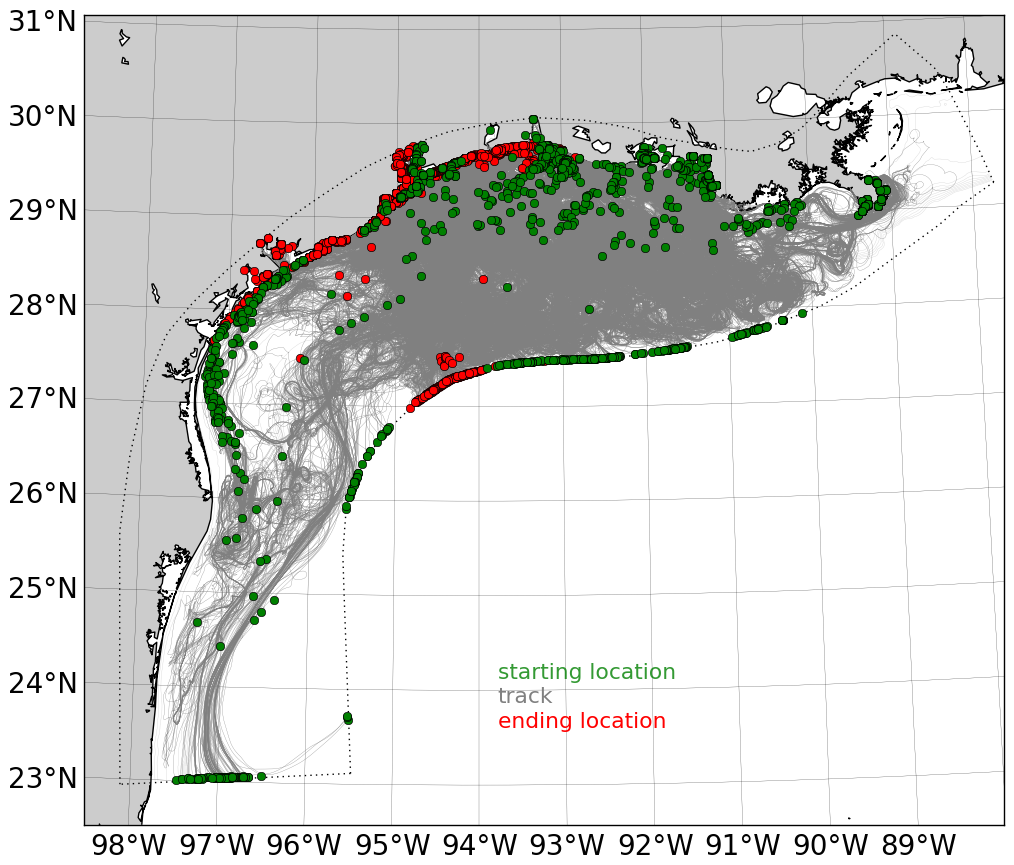
\includegraphics[width=\textwidth]{figures/matt/shelftracks.png}
    \caption{Drifter tracks that move near Galveston Bay and beyond.}
    \label{fig:shelftracks}
\end{figure}

\begin{figure}
    \centering
    \subfigure[Tracks]{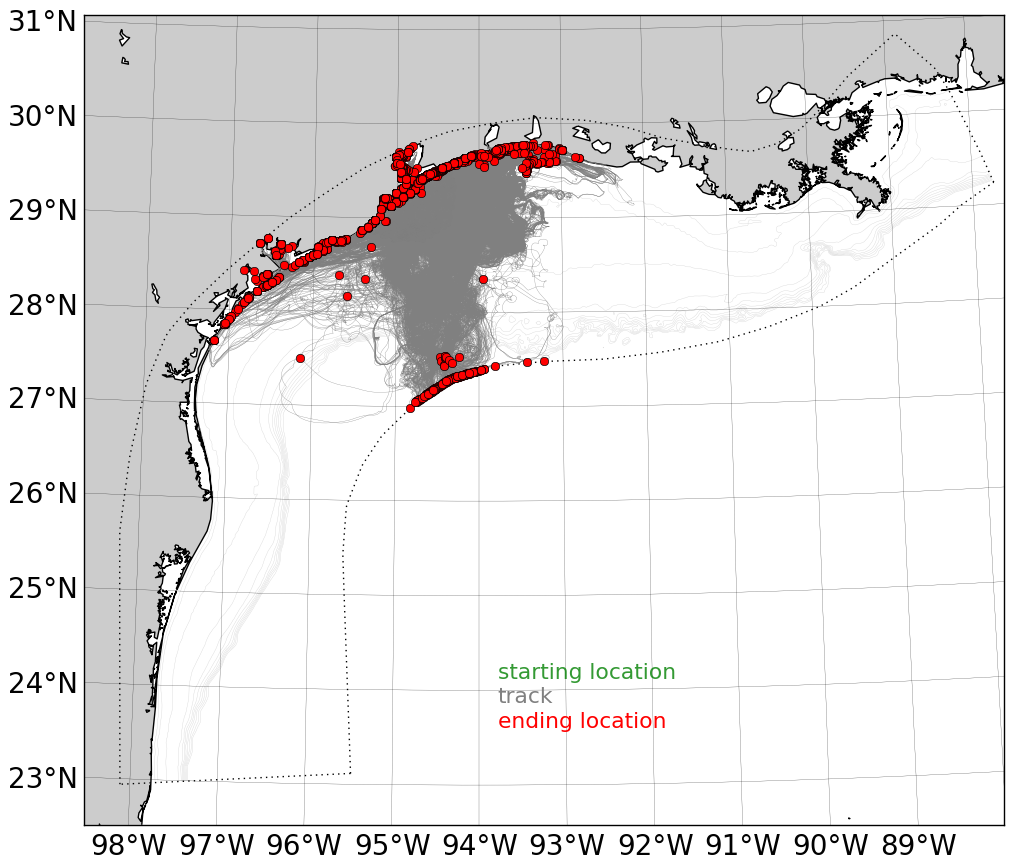
\includegraphics[width=.49\textwidth]{figures/matt/shelf_backonlytracks.png}}
    \subfigure[Transport]{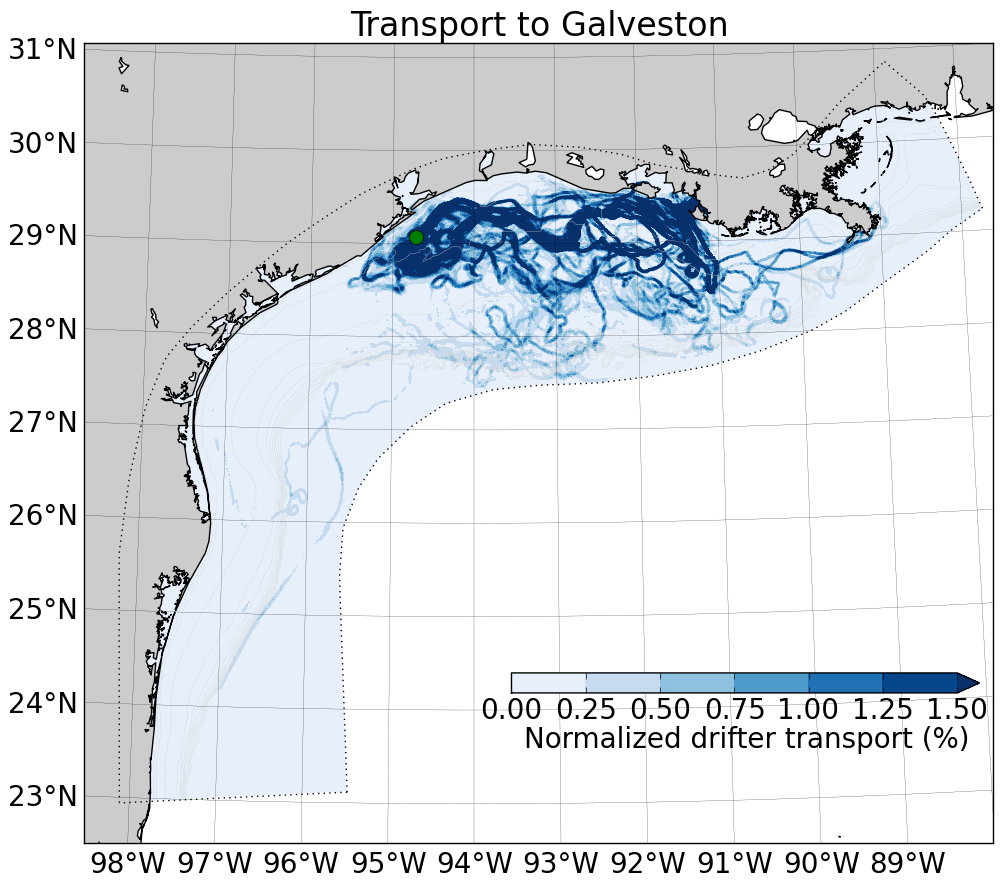
\includegraphics[width=.49\textwidth]{figures/galv_b/transport}}
    \caption{Drifter tracks that move to near Galveston Bay and beyond.}
    \label{fig:galv_b}
\end{figure}

\begin{figure}
    \centering
    \subfigure[Tracks]{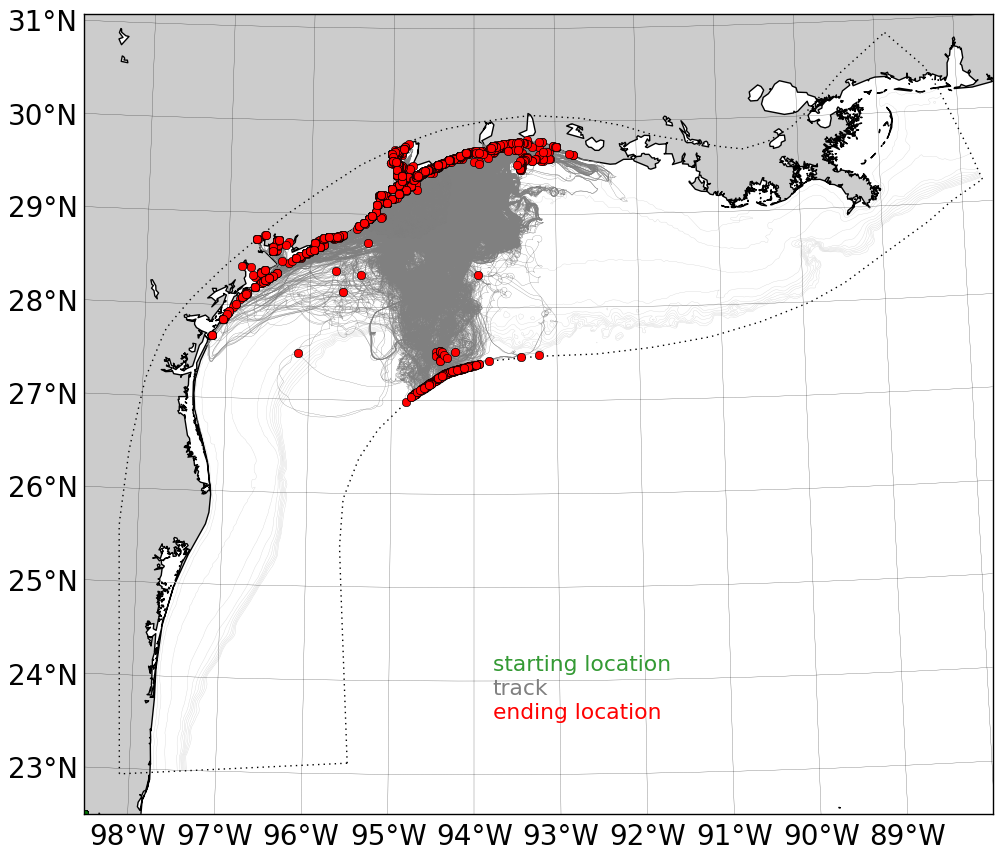
\includegraphics[width=.49\textwidth]{figures/matt/shelf_forwardonlytracks.png}}
    \subfigure[Transport]{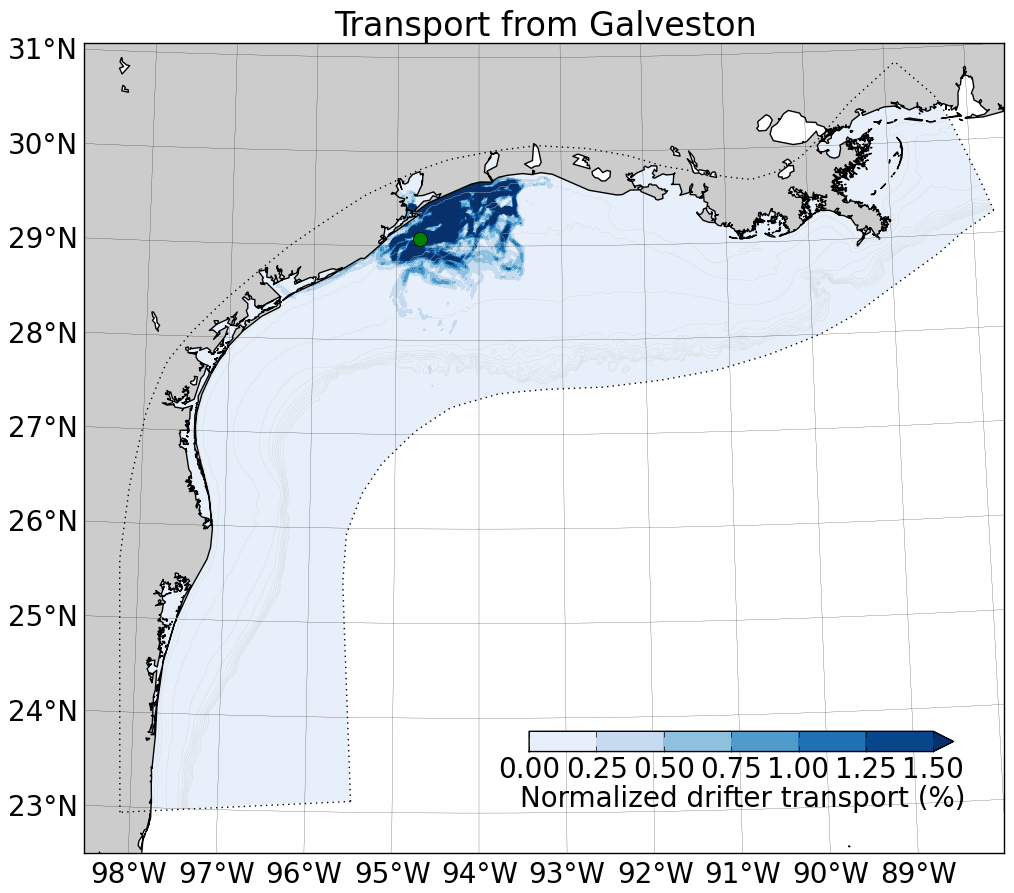
\includegraphics[width=.49\textwidth]{figures/galv_f/transport}}
    \caption{Drifter tracks that move from near Galveston Bay and beyond.}
    \label{fig:galv_f}
\end{figure}

Unfortunately, there are so many tracks that it is hard to tell what is going on, other than that there is a lot going on. Alternatively, separate views of the tracks may be informative. The 90-day backward tracks from near Galveston Bay are shown as tracks and for transport in Figure \ref{fig:galv_b} (see Section \ref{sec:transport} for details on transport). The forward simulations, Figure \ref{fig:galv_f}, are not as dynamic as the backward simulations, but are further studied near the Bay in the next section.

Figures \ref{fig:shelftracks} and \ref{fig:galv_b} show that a wide variety of area can have an effect on Galveston Bay, and this will certainly change with wind conditions.

\subsection{Bay Comparisons}

Tracks moving forward in time from outside Galveston Bay are shown in Figure \ref{fig:baytracks} for the shelf and the Bay models. Drifters in the more highly-resolved SUNTANS Bay model have regular pulsing with the tides, which leads to regular, realistic tracks. The shelf model does not model tides and cannot resolve the complicate channels in the Bay nearly as well, so while drifters are able to make it into the Bay in the shelf model and travel around, more realistic paths are seen in the Bay model.

\begin{figure}
    \centering
    \subfigure[Shelf Model]{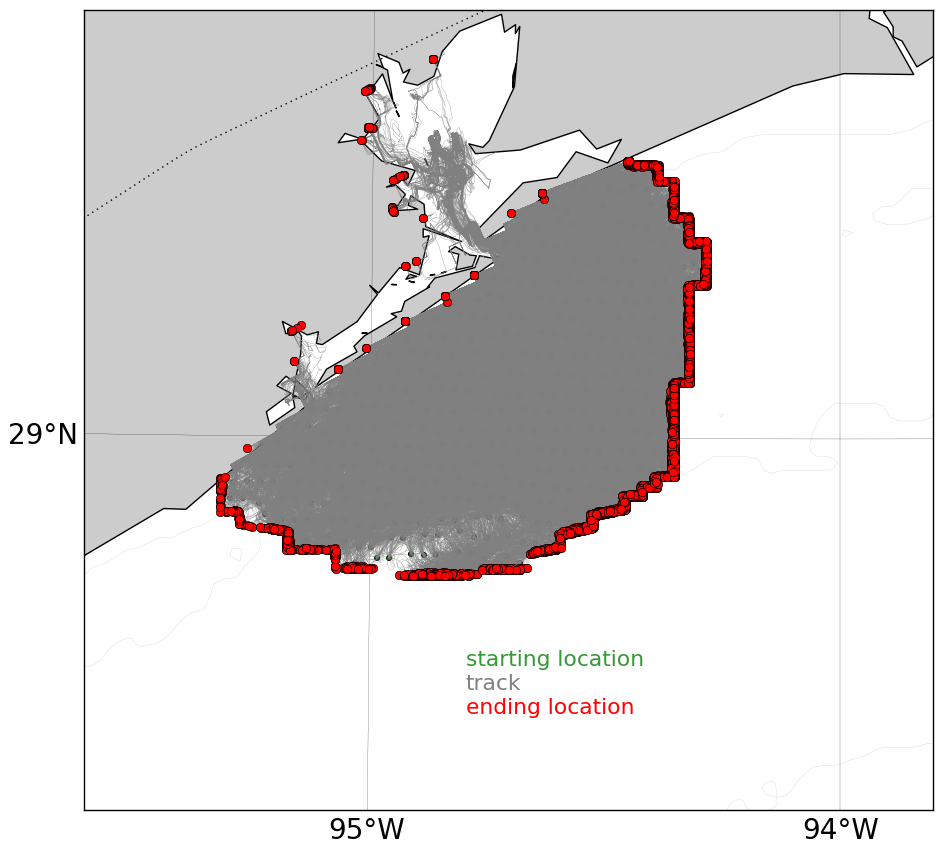
\includegraphics[width=.49\textwidth]{figures/matt/kristentracks.png}}
    \subfigure[Bay Model]{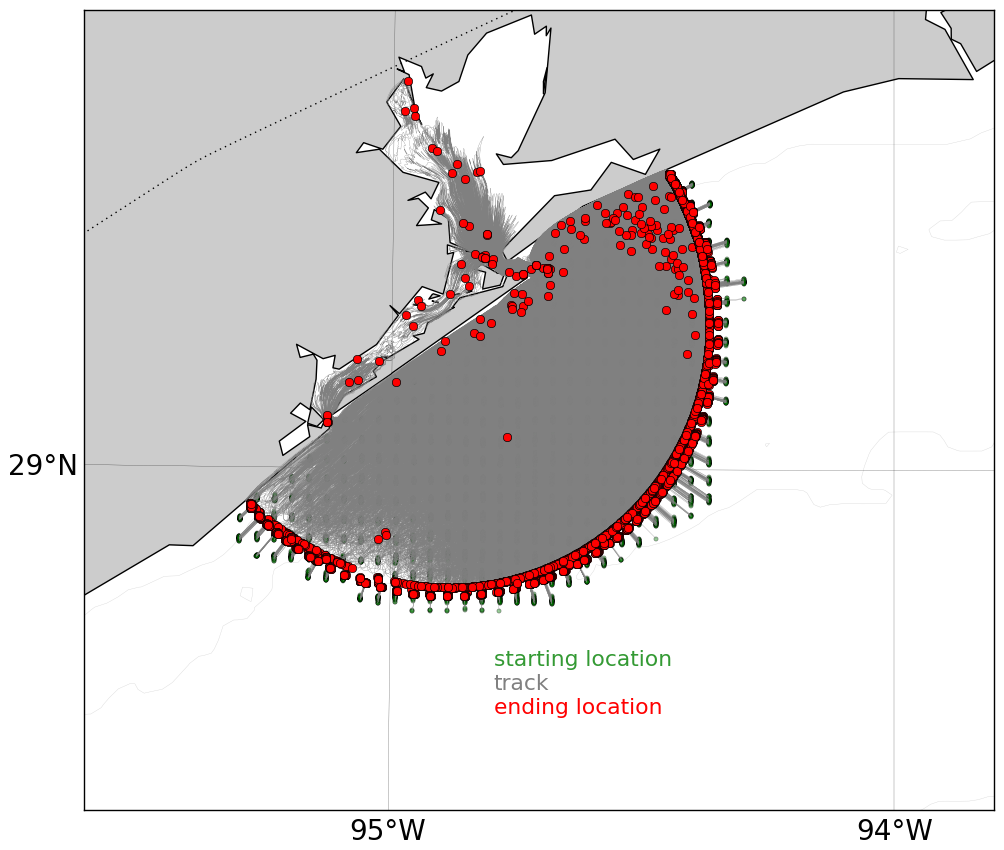
\includegraphics[width=.49\textwidth]{figures/matt/matttracks.png}}
    \caption{Drifter tracks moving forward from outside Galveston Bay for two separate models. Gray lines indicate separate drifter tracks and red circles indicate ending locations after 60 days.}
    \label{fig:baytracks}
\end{figure}

This is also shown in Figure \ref{fig:bayhexbin} in histograms of the drifter final locations that moved forward in time from outside Galveston Bay. The overall behavior is generally the same between the two models, but clearly much more nuanced events occur in the Bay model, leading to more drifters ending up in the Bay and along the western barrier island.

\begin{figure}
    \centering
    \subfigure[Shelf Model]{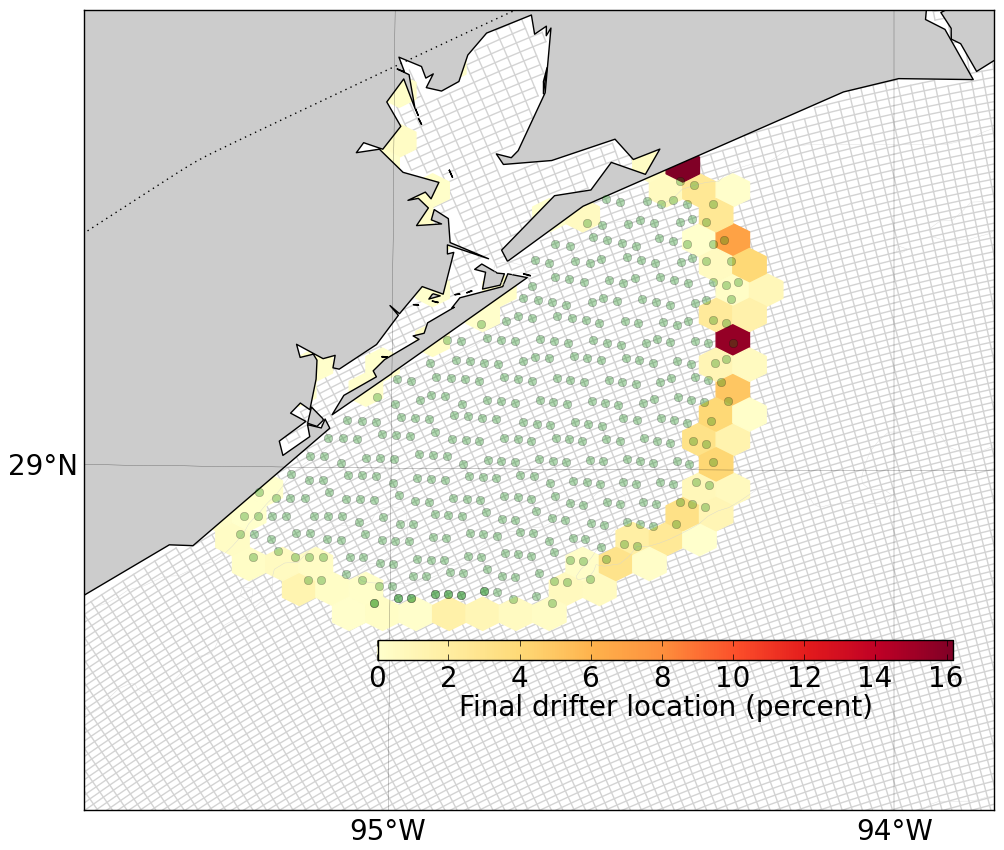
\includegraphics[width=.49\textwidth]{figures/matt/kristenhisthexbin.png}}
    \subfigure[Bay Model]{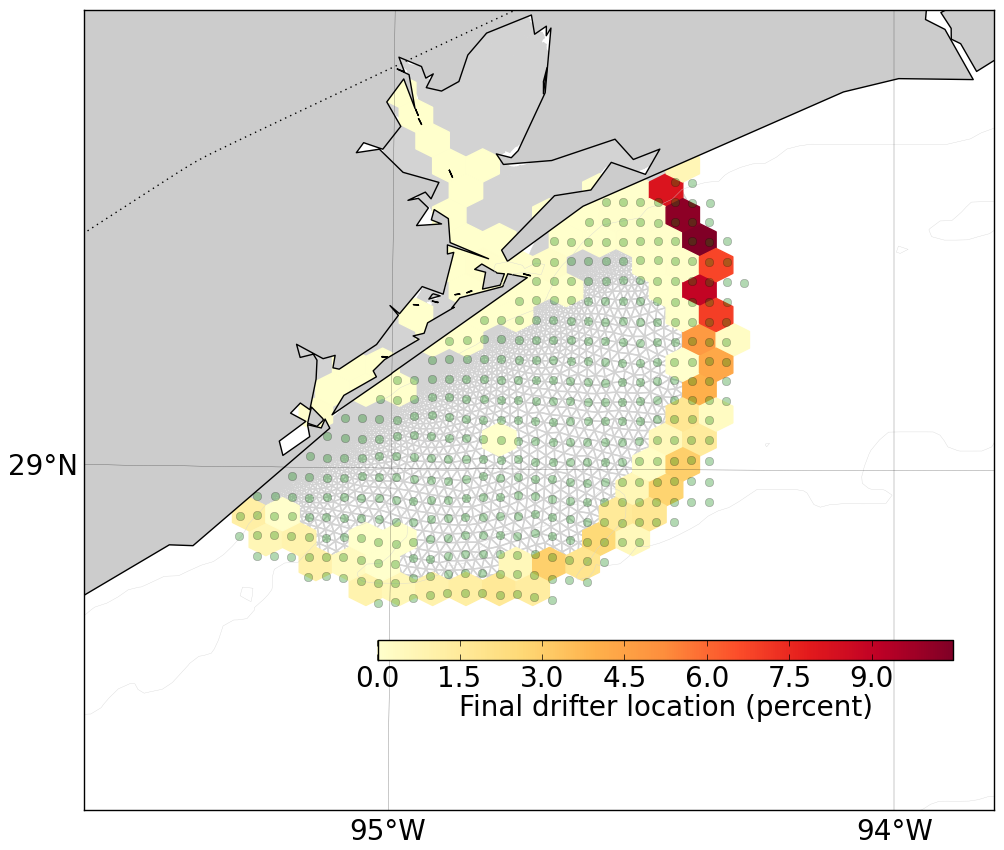
\includegraphics[width=.49\textwidth]{figures/matt/matthisthexbin.png}}
    \caption{Histograms of the final locations of drifters moving forward in time from outside Galveston Bay. Green circles indicate the drifter starting locations and the numerical grid is overlaid for both models.}
    \label{fig:bayhexbin}
\end{figure}

% Now for some results
\section{Results for Different Conditions}

% How do drifters enter Galveston Bay differently for differing weatherbands?
\subsection{Dependence of Circulation on Weatherband}

% Are there major differences in drifter behavior depending on the season, near Galveston Bay?
\subsection{Seasonal Variability}

% What is the connection between behavior near-shore and far-shore?
\subsection{Cross-Shelf Behavior}

% FTLE, LCS, Kirwan
\section{Analysis}

% \begin{figure}
%   \centering
%   \includegraphics[width=.5\textwidth]{figures/domain}
%   \caption{The topography and bathymetry in Admiralty Inlet, with previous data locations shown at Nodule Point and Admiralty Head. The current field data set is at Admiralty Head.}
%   \label{domain}
% \end{figure}

\bibliographystyle{apalike}%abbrv}%plain}
\bibliography{gisr}


\end{document}  